\documentclass[a4paper,10pt]{report}
\usepackage[basque, english]{babel}
\usepackage{listings}

\lstset{
	breaklines=true,
	tabsize=2,
	basicstyle=\ttfamily\small
}

\usepackage{graphicx}
\usepackage{fancyhdr}
\usepackage{caption}

\renewcommand{\chaptername}{Cap\'{i}tulo}
\renewcommand{\contentsname}{Contenido}
% Title Page
\title{Praktika 1: Aktoreak eta filmak kudeatzeko aplikazioa}
\author{Maialen Ruiz Gallo\\Ibon Madariaga Beldarrain\\Endika Perez Larrea\\Marco Alonso Fernandez}


\begin{document}
\maketitle
 
\tableofcontents

%\begin{abstract}
%\end{abstract}

\chapter{Sarrera: Arazoa}

Aplikazio bat garatu nahi da, aktore-kopuru handi bat eta parte hartzen duten filmak kudeatuko dituena. Datuak Wikidatatik jaso dira. Aktore batek film askotan parte har dezake. Era berean, film batean hainbat aktorek lan egin dezakete.



\chapter{Klaseen diseinua}
\begin{figure}[h]
	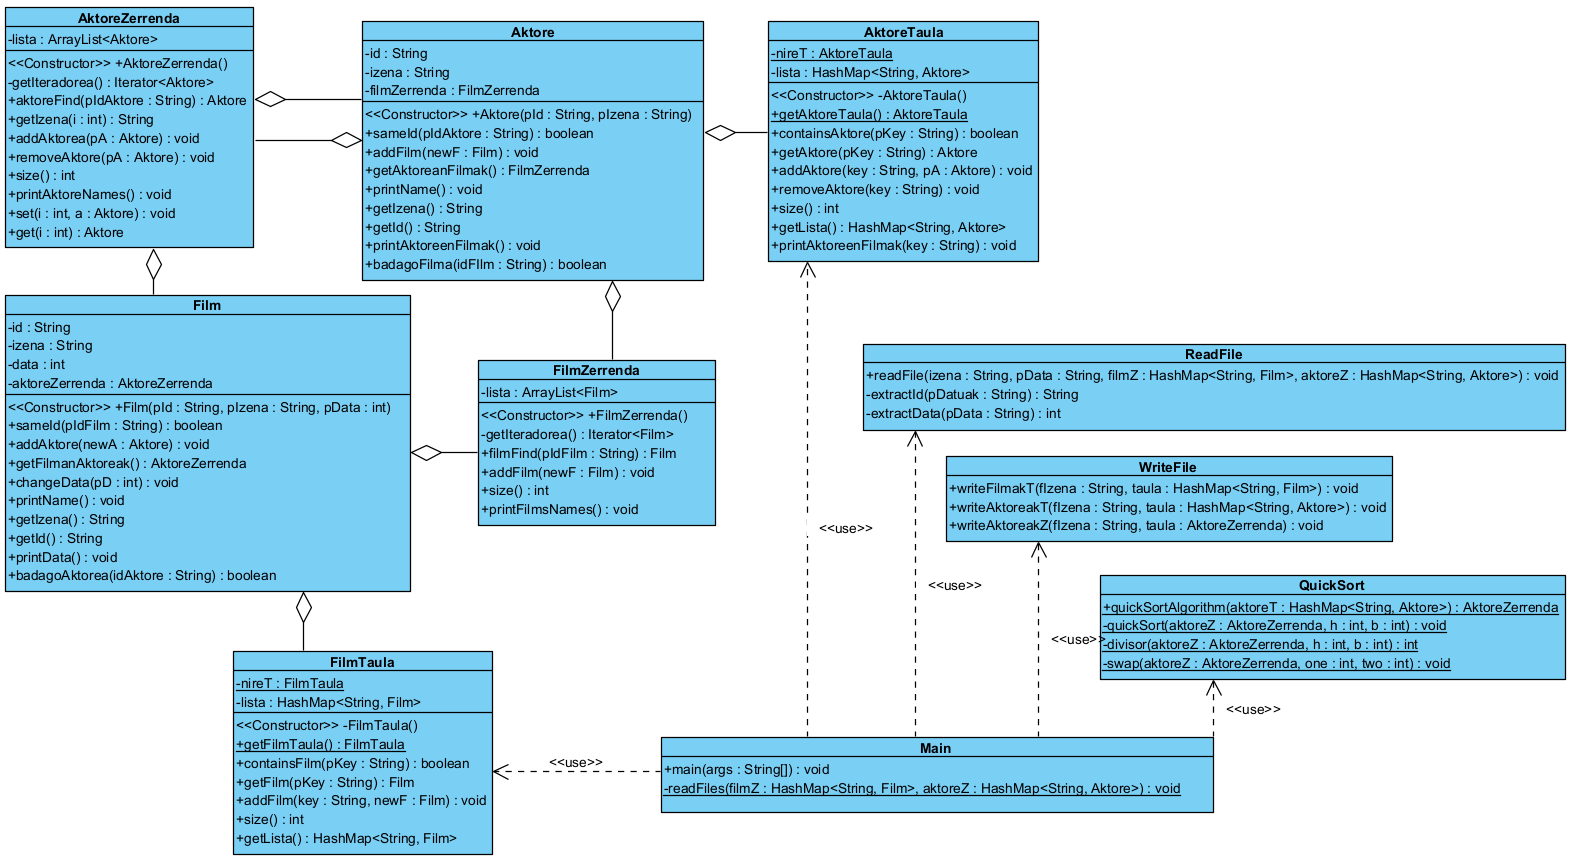
\includegraphics[width=1.3\textwidth]{KlaseDiagramaP1.png}
\end{figure}

\chapter{Datu-egitura nagusien deskribapena}
Aurretik aipatutako arazoa konpontzeko, bi datu-egitura erabili dira: \textit{ArrayList}-ak eta \textit{Hash} taulak.

Hasieran, \textit{ArrayList}-ak erabili ziren soilik, baina algoritmoa ez zen hain eraginkorra. Hori dela eta, \textit{Hash} taula bat erabiltzea erabaki zen.

\section{\textit{ArrayList}}
	\textit{ArrayList} Java-ren datu-egitura bat da, \textit{array}-etatik eratorritakoa. Elementuak elkarren alboan gordeta gelditzen dira memorian eta betetzean, array berri bat sortzen da, tamainaz bikoitza izan ohi dena, eta bertara kopiatzen dira elementu guztiak (orden konstanteko eragiketa da gehienetan, baina betetzean, n-ko kostua du). 

\section{\textit{Hash} taula}
	Hash taulak ere bai arrayetatik datoz. Hash tauletan, elementu bat sartzean, funtzio bat aplikatzen da arrayaren indizea kalkulatzeko eta bertan gordeko da. ArrayListak ez bezala, Hash taulak ez du ordenik bermatzen, hots, ordena alda daiteke.
	
\section{Konparaketa}
	Orokorrean, Hash taulak ArrayListak baino eraginkorragoa da. Esaterako, balio bat bilatzeko, ArrayListean O(n) da eta hash taulan O(1). Hala ere, hash taulak ez du NULL baliorik onartzen. ArrayListek, aldiz, bai.

\chapter{Metodo nagusien diseinua eta implementazioa}
\section{main metodoa}
	\subsection*{Espezifikazioa}
		\begin{itemize}
			\item \textbf{Aurrebaldintza}: Command-Line Argument-ko argumentuak hartzen ditu parametro gisa, baina ez dira erabiltzen. Eclipsek defektuz sortutako metodo izenburua da.
			\item \textbf{Postbaldintza}: Ez du ezer itzultzen
		\end{itemize}
	\subsection*{Kasu-probak}
		\begin{itemize}
			\item Exekuzio arrunta (pelikulen datu base osoarekin)
			\item Exekuzio murriztua (.txt artxibo gutxiekin)
		\end{itemize}
	\subsection*{Deskribapena}
		Metodo hau nagusia da. Bertan, bi hash taula lortzen dira. Horretaz aparte, Quick Sort algoritmoa bertatik deitzen da eta exekuzio-denborak kontrolatu egiten dira.
	\subsection*{Kostua}
		\[
			T(n) = t_{has} + t_{readFiles} + t_{has1} + t_{writeF} + t_{writeAkt} + t_{has2} + t_{QuickSort} + t_{writeSorted} + t_{has3} =
		\]	
		\[
			= K_{1} + t_{readFiles} + t_{writeF} + t_{writeAkt} + t_{QuickSort} + t_{writeSorted} =
		\]
		\[	
			= K_{1} + n*m*(p+q) + f + k + k\log_{2}(k) +k + p =
		\]
		\[	
			= K_{1} + n*m*(p+q) + f + 2k + k\log_{2}(k) + p \in O(n·m·(p + q) + k\log_{2}(k)
		\]
		Kostea kalkulatzeko, batazbesteko kasu hartu da.\\
		Beraz, main metodoaren ordena \textbf{kuasilineala} da.\\
		Kostea kalkulatzeko, hurrengo aldagaiak erabili dira:
		\begin{itemize}
			\item n: Fitxategi kopurua
			\item m: Fitxategi bakoitzeko lerro kopuru handiena
			\item k: Aktore taulan dauden aktoreen kopurua
			\item f: Film taulan dauden film kopurua
			\item p: Aktore batek duen film kopuru handiena
			\item q: Film batek duen aktore kopuru handiena
		\end{itemize}

\section{readFiles metodoa}
	\subsection*{Espezifikazioa}
		\begin{itemize}
			\item \textbf{Aurrebaldintza}: Ez du parametrorik jasotzen.
			\item \textbf{Postbaldintza}: Metodoak ez du ezer itzultzen.
		\end{itemize}
	\subsection*{Kasu-probak}
	\begin{itemize}
		\item Direktorio hutsa (movies-dir karpeta existitzen da, baina ez du artxiborik)
		\item movies-dir karpeta existitzen da, baina .txt ez diren artxiboak ditu
		\item movies-dir karpetak .txt bakarra du
		\item movies-dir karpetak 2 artxibo .txt ditu eta aktore berdina dago bi artxiboetan
		\item Ez da movies-dir karpeta existitzen
	\end{itemize}
	\subsection*{Deskribapena}
		Metodo honek .txt artxibo guztiak array baten barnean sartzen ditu eta artxiboz artxibo irakurtzen ditu.
	\subsection*{Kostua}
		\[
			T(n) = t_{has} + t_{listFiles} + t_{for} = K_{1} + n + n(t_{bald} + t_{readFile}) =
		\]
		\[
			= K_{1} + n + n(K_{2} + m(p+q)) \in O(n*m*(p+q))
		\]
		
		Beraz, readFiles metodoaren ordena \textbf{lineala} da. p eta q txikiak direnez (konstantetzat har daitezke), ordena lineala da $n·m$ lerro kopuruarekiko.\\
		Kostearen kalkuluan n aldagaia erabili da. Bertan, n-k fitxategi kopuruari egiten dio erreferentzia. p eta q aldagaiak erabili dira baita ere: p aktore batek duen film kopuru handienerako eta q film batek  duen aktore kopuru handienerako. Azkenik, m aldagaia erabiltzen da fitxategi bakoitzeko lerro kopuru handiena adierazteko.

\section{readFile metodoa}
	\subsection*{Espezifikazioa}
		\begin{itemize}
			\item \textbf{Aurrebaldintza}: Fitxategiaren "path" osoa (String) eta fitxategiaren izena (String, urtea lortzeko) hartzen ditu parametro gisa.
			\item \textbf{Postbaldintza}: Metodoak ez du ezer itzultzen.
		\end{itemize}
	\subsection*{Kasu-probak}
	\begin{itemize}
		\item Fitxategia ez da existitzen
		\item Fitxategi hutsa
		\item Formatu okerra (datuak ez daude \#\#\#\#-ekin banatuta)
		\item ID eta izena berdinak dira (beraz, ez da gehitu behar)
		\item Aktore berria eta Film berria
		\item Aktorea existitzen da jada, baina filma berria da
		\item Aktore berria, baina filma existitzen da jada
		\item Lerro errepikatua fitxategian
	\end{itemize}
	\subsection*{Deskribapena}
		Metodo hau Main klaseko readFiles metodotik deitzen da iterazio bakoitzean. Bertan, .txt bakoitzaren irakurketa bera burutzen da. Artxiboa lerroz lerro irakurri egiten da, bakoitzetik beharrezko informazioa lortuz eta dagokion lekuak sailkatuz.
	\subsection*{Kostua}
		\[
			T(m) = t_{has1} + t_{while} + t_{has2} = K_{1} + t_{while} =
		\]
		\[
			= K_{1} + m(t_{bald} + t_{badagoF} + t_{badagoAkt}) = K_{1} + m(K_{2} + p + q) \in O(m(p+q))
		\]
		
		Beraz, readFile metodoaren ordena \textbf{lineala} da. p eta q txikiak direnez (konstantetzat har daitezke), ordena lineala da $n·m$ lerro kopuruarekiko.\\
		Kostearen kalkuluan hurrengo aldagaiak erabili dira: m fitxategiaren lerro kopururako, p aktore batek duen film kopuru handienerako eta q film batek  duen aktore kopuru handienerako.

\section{Quick Sort algoritmoa}

	\subsection{quickSortAlgorithm metodoa}
		\subsubsection*{Espezifikazioa}
			\begin{itemize}
				\item \textbf{Aurrebaldintza}: Metodoak aktoreen hash taula hartzen du parametro gisa.
				\item \textbf{Postbaldintza}: Metodoak AktoreZerrenda bat itzultzen du. Bertan, taulako aktore guztiak agertzen dira, ordenatuta.
			\end{itemize}
		\subsubsection*{Kasu-probak}
		\begin{itemize}
			\item Hash mapa hutsa
			\item Hash mapan elementu bakarra
			\item Hash mapan elementu asko eta desordenatuta
		\end{itemize}
		\subsubsection*{Deskribapena}
			Metodo honek algoritmoaren hasieraketak egiten ditu, hala nola, zerrenda berri bat sortu, algoritmoa burutzen duen metodoari deitu eta zerrenda ordenatua itzuli.
		\subsubsection*{Kostua}
			\[
				T(k) = t_{has} + t_{for} + t_{quickSort} + t_{ret} = K_{1} + t_{for} + t_{quickSort} =
			\]
			\[
				= K_{1} + kK_{2} + t_{div} * \log_{2}(k) = K_{1} + kK_{2} + k\log_{2}(k) \in O(k\log_{2}(k))
			\]
			
			Kasu orokorra hartzen bada kontuan (txarrena baino), Quick Sort algoritmoaren ordena \textbf{kuasilineala} da.\\
			Kasu txarrenean (pibotea txikiena edo handiena), ordena \textbf{koadratikoa} da, $O(k^{2})$.\\
			Kostearen kalkuluan k aldagaia erabili da. Bertan, k aktore taulan dauden aktore kopuruari egiten dio erreferentzia.
	
	\subsection{quickSort metodoa}
		\subsubsection*{Espezifikazioa}
			\begin{itemize}
				\item \textbf{Aurrebaldintza}: Metodoak aktore-zerrenda (ordenatze prozesuaren zehar emaitzak jartzen diren zerrenda) eta bi zenbaki oso jasotzen ditu (hasierako eta bukaerako posizioak).
				\item \textbf{Postbaldintza}: Metodoak ez du ezer itzultzen.
			\end{itemize}
		\subsubsection*{Kasu-probak}
		\begin{itemize}
			\item Zerrenda hutsa
			\item Elementu bakarreko zerrenda
			\item Zerrenda bi elementu ordenatuta ditu
			\item Zerrendak bi elementu desordenatuta ditu
			\item Zerrendak hainbat elementu ordenatuta ditu
			\item Zerrendak hainbat elementu desordenatuta ditu
			\item Zerrendak hainbat elementu ditu alderantziz ordenatuta
			\item Zerrendak errepikatzen diren elementuak ditu
		\end{itemize}
		\subsubsection*{Deskribapena}
			Metodo honek quick sort algoritmoa bera burutzen du, dei errekurtsiboekin.
		\subsubsection*{Kostua}
			\[
				T(s) = 2·T(s/2) + s \in O(s\log_{2}(s))
			\]
			
			Beraz, Quick Sort algoritmoaren ordena \textbf{kuasilineala} da.\\
			Kostearen kalkuluan s aldagaia erabili da. Bertan, s zatitu behar den azpizerrendaren tamaina da ($s = b - h + 1$).
	
	\subsection{divisor metodoa}
		\subsubsection*{Espezifikazioa}
			\begin{itemize}
				\item \textbf{Aurrebaldintza}: Metodoak aktore-zerrenda (ordenatze prozesuaren zehar emaitzak jartzen diren zerrenda) eta bi zenbaki oso jasotzen ditu (hasierako eta bukaerako posizioak).
				\item \textbf{Postbaldintza}: "right" izeneko aldagaia itzultzen du indize gisa erabiltzeko.
			\end{itemize}
		\subsubsection*{Kasu-probak}
		\begin{itemize}
			\item Elememtu bakarra (h=b)
			\item Bi elementu ordenatuta
			\item Bi elementu desordenatuta
			\item Pibotea txikiena da (zerrenda jada ordenatua)
			\item Pibotea handiena da (zerrenda alderantziz ordenatua)
			\item Pibotea erdian dago
		\end{itemize}
		\subsubsection*{Deskribapena}
			Metodo honek Quick Sort algoritmoak behin eta berriz egiten duen zatiketa burutzen du.
		\subsubsection*{Kostua}
			\[
				T(s) = t_{has} + t_{while} + t_{ret}= K_{1} + t_{while} = K_{1} + sK_{2} \in O(s)
			\]
			
			Beraz, divisor metodoaren ordena \textbf{lineala} da.\\
			Kostearen kalkuluan s aldagaia erabili da. Bertan, s zatitu behar den azpizerrendaren tamaina da ($s = b - h + 1$).
	
	\subsection{swap metodoa}
		\subsubsection*{Espezifikazioa}
			\begin{itemize}
				\item \textbf{Aurrebaldintza}: Metodoak aktore-zerrenda (ordenatze prozesuaren zehar emaitzak jartzen diren zerrenda) eta bi zenbaki oso jasotzen ditu (trukatu nahi diren bi elementuen posizioak).
				\item \textbf{Postbaldintza}: Metodoak ez du ezer itzultzen.
			\end{itemize}
		\subsubsection*{Kasu-probak}
		\begin{itemize}
			\item Bi elementu ordenatu lekuz aldatu
		\end{itemize}
		Ez dago kasu-proba gehiagorik. Izan ere, metodoari deitu baino lehen aztertzen da lehenengo elementua bigarrena baino txikiagoa dela. Bestela, ez da metodoa deitzen, beraz, hori da aukera bakarra.
		\subsubsection*{Deskribapena}
			Metodo honek bi balioren aldaketa burutzen du, aldagai temporal baten laguntzarekin.
		\subsubsection*{Kostua}
			Kostua \textbf{konstantea} da O(1) edozein posizioko edozein elementurekin denbora berdina behar izango baitu.

\chapter{Kodigoa}
\section{Main klasea}
\begin{lstlisting}[language=Java]
    package packLaboTaula;
    
    import java.io.File;
    
    public class Main {
    	
    	public static void main(String[] args) {
    		long start = System.currentTimeMillis();
    		//ALGORITMO NAGUSIA
    		AktoreTaula aktoreZ = AktoreTaula.getAktoreTaula();
    		FilmTaula filmZ = FilmTaula.getFilmTaula();
    		readFiles();
    		//EXEKUZIO DENBORA: ALGORITMO NAGUSIA
    		long end = System.currentTimeMillis();
    		double exTime = (double) ((end - start)/1000);
    		
    		//PRINT-AK
    		System.out.println("===PRINT===\n");
    		System.out.println("execution time - algoritmo nagusia: " + exTime + " seconds");
    		System.out.println("AktoreZ  " + aktoreZ.size());
    		System.out.println("FilmZ  " + filmZ.size());
    		System.out.println("");
    		//IDAZKETA
    		WriteFile writeFile = new WriteFile();
    		writeFile.writeFilmakT("filmak.txt", FilmTaula.getFilmTaula());
    		writeFile.writeAktoreakT("aktoreak.txt", AktoreTaula.getAktoreTaula());
    		
    		//SORT
    		System.out.println("===SORT===\n");
    		start = System.currentTimeMillis();
    		AktoreZerrenda aktoreSorted = QuickSort.quickSortAlgorithm(aktoreZ.getLista());
    		writeFile.writeAktoreakZ("aktoreakSorted.txt", aktoreSorted);
    		end = System.currentTimeMillis();
    		exTime = (double) ((end - start)/100);
    		System.out.println("execution time - quick sort: " + exTime + " mili seconds");
    		System.out.println("");
    		
    		//PROBAK
    		System.out.println("===PROBAK===\n");
    		aktoreZ.printAktoreenFilmak("HarrisonFordQ81328");
    		System.out.println("");
    		aktoreZ.printAktoreenFilmak("HarryStylesQ3626966");
    		System.out.println("");
    		aktoreZ.printAktoreenFilmak("ZendayaQ189489");
    	}
    	
    	private static void readFiles() {
    		File directory = new File("src/packLaboTaula/movies-dir/");
    		File[] files = directory.listFiles();
    		ReadFile reader = new ReadFile();
    		for(File file : files) {
    			if (file.isFile() && file.getName().endsWith(".txt")) 
    			reader.readFile(file.getAbsolutePath(), file.getName());
    		}
    	}
    }
\end{lstlisting}

\section{ReadFile klasea}
\begin{lstlisting}[language=java]
	package packLaboTaula;
	
	import java.io.FileReader;
	import java.io.IOException;
	import java.util.Scanner;
	
	public class ReadFile {
		public void readFile(String izena, String pData) {
			try {
				Scanner sarrera = new Scanner(new FileReader(izena));
				int data = extractData(pData);
				while (sarrera.hasNext()) {
					String[] datuak = sarrera.nextLine().split("\\s+###\\s+");
					if (datuak.length != 4) continue;
					String aktoreId = extractId(datuak[0]);
					String aktoreIzena = datuak[1];
					String filmId = extractId(datuak[2]);
					String filmIzena = datuak[3];
					
					if (aktoreId.equals(aktoreIzena) || filmId.equals(filmIzena)) continue;
					
					String aktoreKey = aktoreIzena.replace(" ", "").concat(aktoreId);
					String filmKey = filmIzena.replace(" ", "").concat(filmId);
					
					Aktore aktore = AktoreTaula.getAktoreTaula().getAktore(aktoreKey);
					if (aktore == null) {
						aktore = new Aktore(aktoreId, aktoreIzena);
						AktoreTaula.getAktoreTaula().addAktore(aktoreKey, aktore);
					}
					
					Film film = FilmTaula.getFilmTaula().getFilm(filmKey);
					if (film == null) {
						film = new Film(filmId, filmIzena, data);
						FilmTaula.getFilmTaula().addFilm(filmKey, film);
					}
					
					if(!aktore.badagoFilma(filmId)) aktore.addFilm(film);
					if(!film.badagoAktorea(aktoreId)) film.addAktore(aktore);   
				}
				sarrera.close();
			} // try 
			catch (IOException e) {
				e.printStackTrace();
			}                                 
		}
		
		private String extractId(String pDatuak) {
			String[] datuak = pDatuak.split("/");
			return (datuak[4]);
		}
		
		private int extractData(String pData) {
			
			String[] dataSplit = pData.split("_");
			String[] dataSplit2 = dataSplit[3].split("\\.");
			int data = Integer.parseInt(dataSplit2[0]);
			return data;
		}
	}
\end{lstlisting}

\section{WriteFile klasea}
\begin{lstlisting}[language=java]
	package packLaboTaula;
	
	import java.io.IOException;
	import java.io.PrintWriter;
	
	public class WriteFile {
		public void writeFilmakT(String fIzena, FilmTaula filmTaula) {
			try {
				PrintWriter writer = new PrintWriter(fIzena, "UTF-8");
				for (Film film : filmTaula.getLista().values())
				writer.printf("%-60s  %s%n", film.getIzena(), film.getId());
				writer.close();
			}
			catch (IOException e) {
				e.printStackTrace();
			}
		}
		
		public void writeAktoreakT(String fIzena, AktoreTaula aktoreTaula) {
			try {
				PrintWriter writer = new PrintWriter(fIzena, "UTF-8");
				for (Aktore aktore : aktoreTaula.getLista().values())
				writer.printf("%-60s  %s%n", aktore.getIzena(), aktore.getId());
				writer.close();
			}
			catch (IOException e) {
				e.printStackTrace();
			}
		}
		
		public void writeAktoreakZ(String fIzena, AktoreZerrenda taula) {
			try {
				PrintWriter writer = new PrintWriter(fIzena, "UTF-8");
				for (int i = 0; i < taula.size() ; i++)
				writer.printf("%-60s  %s%n", taula.get(i).getIzena(), taula.get(i).getId());
				writer.close();
			}
			catch (IOException e) {
				e.printStackTrace();
			}
		}
	}
\end{lstlisting}

\section{QuickSort klasea}
\begin{lstlisting}[language=java]
	package packLaboTaula;
	
	import java.util.HashMap;
	
	public class QuickSort {
		
		public static AktoreZerrenda quickSortAlgorithm(HashMap<String, Aktore> AktoreT) {
			AktoreZerrenda sortedList = new AktoreZerrenda();
			for (String key: AktoreT.keySet()) {
				sortedList.addAktorea(AktoreT.get(key));
			}
			//System.out.print(sortedList.getIzena(0) +"     "+ sortedList.getIzena(1));
			//System.out.print(sortedList.getIzena(0).compareTo(sortedList.getIzena(1)));
			quickSort(sortedList, 0, sortedList.size()-1);
			return sortedList;
		}
		
		private static void quickSort(AktoreZerrenda aktoreZ, int h, int b) {
			if (b-h > 0) {
				int index = divisor(aktoreZ, h, b);
				quickSort(aktoreZ, h, index-1);
				quickSort(aktoreZ, index+1, b);
			}
		}
		
		private static int divisor(AktoreZerrenda aktoreZ, int h, int b) {
			Aktore tempAktore = aktoreZ.get(h);
			String tempIzena = aktoreZ.getIzena(h);
			int left = h;
			int right = b;
			while (left < right) {
				while (aktoreZ.getIzena(left).compareTo(tempIzena) <= 0 && left < right)
				left++;
				while (aktoreZ.getIzena(right).compareTo(tempIzena) > 0 && left < right)
				right--;
				if (left < right)
				swap(aktoreZ, left, right);
			}
			if (aktoreZ.getIzena(right).compareTo(tempIzena) > 0)
			right--;
			aktoreZ.set(h, aktoreZ.get(right));
			aktoreZ.set(right, tempAktore);
			return right;
		}
		
		private static void swap(AktoreZerrenda aktoreZ, int one, int two) {
			Aktore tempAktore = aktoreZ.get(one);
			aktoreZ.set(one, aktoreZ.get(two));
			aktoreZ.set(two, tempAktore);
		}	
	}
\end{lstlisting}

\section{FilmZerrenda klasea}
\begin{lstlisting}[language=java]
	package packLaboTaula;
	
	import java.util.ArrayList;
	import java.util.Iterator;
	
	public class FilmZerrenda {
		private ArrayList<Film> lista;
		
		public FilmZerrenda() {
			this.lista = new ArrayList<Film>(); 
		}
		
		private Iterator<Film> getIteradorea(){
			return this.lista.iterator();
		}
		
		public Film filmFind(String pIdFilm)
		{
			Film filmFound = null;
			Film f = null;
			Iterator<Film> itr = this.getIteradorea();
			while(itr.hasNext() && filmFound == null) {
				f = itr.next();
				if (f.sameId(pIdFilm))
				filmFound = f;
			}
			return filmFound;
		}
		
		public void addFilm(Film newF) {
			this.lista.add(newF);
		}
		
		public int size() {
			return this.lista.size();
		}
		
		public void printFilmsNames() {
			Film f = null;
			Iterator<Film> itr = this.getIteradorea();
			while(itr.hasNext()) {
				f = itr.next();
				System.out.print("    ");
				f.printName();
				System.out.print("    ");
				f.printData();
				System.out.println();
			}
			
		}
	}
\end{lstlisting}

\section{FilmTaula klasea}
\begin{lstlisting}[language=java]
	package packLaboTaula;
	
	import java.util.HashMap;
	
	public class FilmTaula {
		private static FilmTaula nireT = null;
		private HashMap<String, Film> lista;
		
		private FilmTaula() {
			this.lista = new HashMap<String, Film>(); 
		}
		
		public static FilmTaula getFilmTaula() {
			if (nireT == null)
			nireT = new FilmTaula();
			return nireT;
		}
		
		public boolean conteinsFilm(String pKey)
		{
			return lista.containsKey(pKey);
		}
		
		public Film getFilm(String pKey) {
			return this.lista.get(pKey);
		}
		
		public void addFilm(String key, Film newF) {
			this.lista.put(key, newF);
		}
		
		public int size() {
			return this.lista.size();
		}
		
		public HashMap<String, Film> getLista(){
			return this.lista;
		}
	}
\end{lstlisting}

\section{Film klasea}
\begin{lstlisting}[language=java]
	package packLaboTaula;
	
	public class Film {
		private String id, izena;
		private int data;
		private AktoreZerrenda aktoreZerrenda;
		
		public Film(String pId, String pIzena, int pData) {
			this.id = pId;
			this.izena = pIzena;
			this.data = pData;
			this.aktoreZerrenda = new AktoreZerrenda();
		}
		
		public boolean sameId(String pIdFilm) {
			if (this.id.equals(pIdFilm))
			return true;
			return false;
		}
		
		public void addAktore(Aktore newA) {
			this.aktoreZerrenda.addAktorea(newA);	
		}
		
		public AktoreZerrenda getFilmanAktoreak() {
			return this.aktoreZerrenda;
		}
		
		public void changeData(int pD) {
			this.data = pD;
		}
		
		public void printName() {
			System.out.print(this.izena);
		}
		
		public String getIzena() {
			return this.izena ;
		}
		
		public String getId() {
			return this.id ;
		}
		
		public void printData() {
			System.out.print(this.data);
		}
		
		public boolean badagoAktorea(String idAktore) {
			if (this.aktoreZerrenda.aktoreFind(idAktore) != null)
			return true;
			return false;
		}
		
		public int getData() {
			return this.data;
		}
		
	}
\end{lstlisting}

\section{AktoreZerrenda klasea}
\begin{lstlisting}[language=java]
	package packLaboTaula;
	
	import java.util.ArrayList;
	import java.util.Iterator;
	
	public class AktoreZerrenda {
		private ArrayList<Aktore> lista;
		
		public AktoreZerrenda() {
			this.lista = new ArrayList<Aktore>(); 
		}
		
		private Iterator<Aktore> getIteradorea(){
			return this.lista.iterator();
		}
		
		public Aktore aktoreFind(String pIdAktore)
		{
			Aktore aktoreFound = null;
			Aktore f = null;
			Iterator<Aktore> itr = this.getIteradorea();
			while(itr.hasNext() && aktoreFound == null) {
				f = itr.next();
				if (f.sameId(pIdAktore))
				aktoreFound = f;
			}
			return aktoreFound;
		}
		
		public String getIzena(int i) {
			return this.lista.get(i).getIzena();
		}
		
		public void addAktorea(Aktore pA) {
			this.lista.add(pA);
		}
		
		public void removeAktore(Aktore pA) {
			this.lista.remove(pA);
		}
		
		public int size() {
			return this.lista.size();
		}
		
		public void printAktoreNames() {
			Aktore f = null;
			Iterator<Aktore> itr = this.getIteradorea();
			while(itr.hasNext()) {
				f = itr.next();
				f.printName();
			}
		}
		
		public void set(int i, Aktore a) {
			this.lista.set(i, a);
		}
		
		public Aktore get(int i) {
			return this.lista.get(i);
		}
		
	}
\end{lstlisting}

\section{AktoreTaula klasea}
\begin{lstlisting}[language=java]
	package packLaboTaula;
	
	import java.util.HashMap;
	
	public class AktoreTaula {
		private static AktoreTaula nireT = null;
		private HashMap<String, Aktore> lista;
		
		private AktoreTaula() {
			this.lista = new HashMap<String, Aktore>(); 
		}
		
		public static AktoreTaula getAktoreTaula() {
			if (nireT == null)
			nireT = new AktoreTaula();
			return nireT;
		}
		
		public boolean conteinsAktore(String pKey)
		{
			if (this.lista.containsKey(pKey)) return true;
			else return false;
		}
		
		public Aktore getAktore(String pKey) {
			return this.lista.get(pKey);
		}
		
		public void addAktore(String key, Aktore pA) {
			this.lista.put(key, pA);
		}
		
		public void removeAktore(String key) {
			this.lista.remove(key);
		}
		
		public int size() {
			return this.lista.size();
		}
		
		public HashMap<String, Aktore> getLista() {
			return lista;
		}
		
		public void printAktoreenFilmak(String key) {
			this.lista.get(key).printAktoreenFilmak();
		}
		
	}
\end{lstlisting}
\section{Aktore klasea}
\begin{lstlisting}[language=java]
	package packLaboTaula;
	
	public class Aktore {
		private String id, izena;
		private FilmZerrenda filmZerrenda;
		
		public Aktore(String pId, String pIzena) {
			this.id = pId;
			this.izena = pIzena;
			this.filmZerrenda = new FilmZerrenda();
		}
		
		public boolean sameId(String pIdAktore) {
			if (this.id.equals(pIdAktore))
			return true;
			return false;
		}
		
		public void addFilm(Film newF) {
			this.filmZerrenda.addFilm(newF);
		}
		
		public FilmZerrenda getAktoreanFilmak() {
			return this.filmZerrenda;
		}
		
		public void printName() {
			System.out.println(this.izena);
		}
		
		public String getIzena() {
			return this.izena;
		}
		
		public String getId() {
			return this.id;
		}
		
		public void printAktoreenFilmak() {
			System.out.println(this.izena + ":");
			this.filmZerrenda.printFilmsNames();
		}
		
		public boolean badagoFilma(String idFilm) {
			if (this.filmZerrenda.filmFind(idFilm) != null)
			return true;
			return false;
		}
	}
\end{lstlisting}

\section{JUNIT klaseak}
	\subsection{AktoreTest klasea}
\begin{lstlisting}[language=java]
	package packLaboTaula;
	
	import static org.junit.jupiter.api.Assertions.*;
	import org.junit.jupiter.api.Test;
	
	class AktoreTest {
		
		Aktore a = new Aktore("QR6767", "Ramon");
		Aktore b = new Aktore("QR6767", "Ignacio");
		Film f = new Film("QT3333","Frankenstein",1967);
		
		//Hacer esto pero en varios @Test, importante
		@Test
		void testGetIzena() {
			assertEquals("Ramon", a.getIzena());	
		}
		
		@Test
		void testGetId() {
			assertEquals("QR6767", a.getId());
		}
		
		@Test
		void getAktoreanFilmakNotNull() {
			assertNotNull(a.getAktoreanFilmak());		
		}
		
		@Test
		void testSameId() {		
			assertTrue(a.sameId(b.getId()));
		}
		
		@Test
		void testAddFilm() {
			a.addFilm(f);
			assertEquals(a.getAktoreanFilmak().size(),1);
		}
		
		@Test
		void testBadagoFilma() {	
			a.addFilm(f);
			assertTrue(a.badagoFilma(f.getId()));
		}
	}
\end{lstlisting}

	\subsection{AktoreZerrendaTest klasea}
\begin{lstlisting}[language=java]
	package packLaboTaula;
	
	import static org.junit.jupiter.api.Assertions.*;
	
	import org.junit.jupiter.api.Test;
	
	class AktoreZerrendaTest {
		
		AktoreZerrenda az = new AktoreZerrenda();
		Aktore a = new Aktore("QR6767","Ramon");
		Aktore a2 = new Aktore("QR6869","Andeka");
		
		@Test
		void testAddAktore() {
			az.addAktorea(a);
			assertEquals(az.size(),1);
		}
		
		@Test
		void testRemoveAktore() {
			az.addAktorea(a);
			az.removeAktore(a);
			assertEquals(az.size(),0);
		}
		
		@Test
		void testAktoreFind() {
			az.addAktorea(a);
			assertEquals(az.aktoreFind(a.getId()),a);
		}
		
		@Test
		void testGet() {
			az.addAktorea(a);
			assertEquals(az.get(0),a);
		}
		
		@Test
		void testSet() {
			az.addAktorea(a);
			az.addAktorea(a2);
			az.set(1, a);
			assertEquals(az.get(1),a);
		}
		
	}
\end{lstlisting}

	\subsection{AktoreTaulaTest klasea}
\begin{lstlisting}[language=java]
	package packLaboTaula;
	
	import static org.junit.jupiter.api.Assertions.*;
	
	import java.util.HashMap;
	
	import org.junit.jupiter.api.Test;
	
	class AktoreTaulaTest {
		
		Aktore a = new Aktore("QR6767","Ramon");
		
		@Test
		void testGetAktoreTaula() {
			assertNotNull(AktoreTaula.getAktoreTaula());
		}
		
		@Test
		void testSize() {
			assertEquals(0, AktoreTaula.getAktoreTaula().size());
		}
		
		@Test
		void testAddAktore() {
			AktoreTaula.getAktoreTaula().addAktore(a.getId(), a);
			assertEquals(1, AktoreTaula.getAktoreTaula().size());
		}
		
		@Test
		void testRemoveAktore() {
			AktoreTaula.getAktoreTaula().addAktore(a.getId(), a);
			AktoreTaula.getAktoreTaula().removeAktore(a.getId());
			assertEquals(0, AktoreTaula.getAktoreTaula().size());
		}
		
		@Test
		void testConteinsAktore() {
			AktoreTaula.getAktoreTaula().addAktore(a.getId(), a);
			assertTrue(AktoreTaula.getAktoreTaula().conteinsAktore(a.getId()));
		}
		
		@Test
		void testGetLista() {
			HashMap<String, Aktore> lista = AktoreTaula.getAktoreTaula().getLista();
			assertNotNull(lista);
		}
		
	}
\end{lstlisting}

	\subsection{FilmTest klasea}
\begin{lstlisting}[language=java]
	package packLaboTaula;
	
	import static org.junit.jupiter.api.Assertions.*;
	import org.junit.jupiter.api.Test;
	
	class FilmTest {
		
		Film f = new Film("QL6869","La Momia", 1998);
		Film f2 = new Film("QL6869","American History X", 1998);
		Aktore a = new Aktore("QR6767","Ramon");
		
		//Hacer esto pero en varios @Test, importante para saber donde es el fallo en caso de haber uno
		
		@Test
		void testGetIzena() {
			assertEquals("La Momia", f.getIzena());
		}
		
		@Test
		void testGetId() {
			assertEquals("QL6869", f.getId());		
		}
		
		@Test
		void testGetFilmanAktoreakNotNull() {
			assertNotNull(f.getFilmanAktoreak());		
		}
		
		@Test
		void testSameId() {
			assertTrue(f.sameId(f2.getId()));		
		}
		
		@Test
		void testAddAktore() {
			f.addAktore(a);
			assertEquals(f.getFilmanAktoreak().size(),1);
		}
		
		@Test
		void testBadagoAktorea() {
			f.addAktore(a);		
			assertTrue(f.badagoAktorea(a.getId()));
		}
		
		@Test
		void testGetData() {
			assertEquals(f.getData(), 1998);		
		}
	}
\end{lstlisting}

	\subsection{FilmZerrendaTest klasea}
\begin{lstlisting}[language=java]
	package packLaboTaula;
	
	import static org.junit.jupiter.api.Assertions.*;
	
	import org.junit.jupiter.api.Test;
	
	class FilmZerrendaTest {
		
		FilmZerrenda fz = new FilmZerrenda();
		Film f = new Film("QL6869","American History X", 1998);
		
		@Test
		void testSize() {
			assertEquals(fz.size(),0);
		}
		
		@Test
		void testAddFilm() {
			fz.addFilm(f);
			assertEquals(fz.size(),1);
		}
		
		@Test
		void testFilmFind() {
			fz.addFilm(f);
			assertEquals(fz.filmFind(f.getId()),f);
		}
	}
\end{lstlisting}

	\subsection{FilmTaulaTest klasea}
\begin{lstlisting}[language=java]
	package packLaboTaula;
	
	import static org.junit.jupiter.api.Assertions.*;
	
	import java.util.HashMap;
	
	import org.junit.jupiter.api.Test;
	
	class FilmTaulaTest {
		
		Film f = new Film("QL6869","American History X", 1998);
		Film f2 = new Film("QL6870","La Momia", 1998);
		
		@Test
		void testGetFilmTaula() {
			assertNotNull(FilmTaula.getFilmTaula());
		}
		
		@Test
		void testAddFilm() {
			FilmTaula.getFilmTaula().addFilm(f.getId(), f);
			FilmTaula.getFilmTaula().addFilm(f2.getId(), f2);
			assertEquals(FilmTaula.getFilmTaula().size(),2);
		}
		
		@Test
		void testGetFilm() {
			FilmTaula.getFilmTaula().addFilm(f.getId(), f);
			assertEquals(FilmTaula.getFilmTaula().getFilm(f.getId()),f);
		}
		
		@Test
		void testConteinsFilm() {
			FilmTaula.getFilmTaula().addFilm(f.getId(), f);
			assertTrue(FilmTaula.getFilmTaula().conteinsFilm(f.getId()));
		}
		
		@Test
		void testGetLista() {
			HashMap<String, Film> lista = FilmTaula.getFilmTaula().getLista();
			assertNotNull(lista);
		}	
	}
\end{lstlisting}
	\subsection{QuickSortTest klasea}
\begin{lstlisting}[language=java]
	package packLaboTaula;
	
	import static org.junit.jupiter.api.Assertions.*;
	
	import java.util.HashMap;
	
	import org.junit.jupiter.api.Test;
	
	class QuickSortTest {
		
		@Test
		void testQuickSortHutsa() {
			HashMap<String, Aktore> map = new HashMap<>();
			
			AktoreZerrenda r = QuickSort.quickSortAlgorithm(map);
			assertEquals(0, r.size());
		}
		
		@Test
		void testQuickSortElementuBakarra() {
			HashMap<String, Aktore> map = new HashMap<>();
			
			map.put("QR6767", new Aktore("QR6767", "Ramon"));
			
			AktoreZerrenda r = QuickSort.quickSortAlgorithm(map);
			
			assertEquals(1, r.size());
			assertEquals("Ramon", r.getIzena(0));
		}
		
		@Test
		void testQuickSortHainbatElementu() {
			
			HashMap<String, Aktore> map = new HashMap<>();
			
			map.put("1", new Aktore("1", "Mikel"));
			map.put("2", new Aktore("2", "Ana"));
			map.put("3", new Aktore("3", "Jon"));
			map.put("4", new Aktore("4", "Bea"));
			
			AktoreZerrenda r = QuickSort.quickSortAlgorithm(map);
			
			assertEquals("Ana", r.getIzena(0));
			assertEquals("Bea", r.getIzena(1));
			assertEquals("Jon", r.getIzena(2));
			assertEquals("Mikel", r.getIzena(3));
		}
		
		@Test
		void testQuickSortAlderantzizkoa() {
			
			HashMap<String, Aktore> map = new HashMap<>();
			
			map.put("1", new Aktore("1", "Zoe"));
			map.put("2", new Aktore("2", "Mikel"));
			map.put("3", new Aktore("3", "Ana"));
			
			AktoreZerrenda r = QuickSort.quickSortAlgorithm(map);
			
			assertEquals("Ana", r.getIzena(0));
			assertEquals("Mikel", r.getIzena(1));
			assertEquals("Zoe", r.getIzena(2));
		}
	}
\end{lstlisting}

\chapter{Konklusioak}
Lan honen bidez argi gelditu da eraginkortasun-aldaketa nabaria dagoela ArrayListen ordez Hash taulak erabiltzen badira. Hura justifikatzeko, programaren bitartez jasotako datuak aurkeztuko dira.

Lehenik, ArrayListaren eta Hash taularen arteko konparaketa ikusiko da. Horretarako, bakoitzaren exekuzio-denbora neurtu da hurrengoa egitean: sortu, fitxategi bakoitza irakurri eta zerrendan/taulan gehitu ez egotekotan.

Bigarrenik, Quick Sort algoritmoaren efizientzia neurtu da. Horretarako, behin taula eginda dagoela, bost proba burutu dira zerrenda ordenatu bat sortzeko eta haien exekuzio-denbora neurtu da.

\section{Saiakerak eta emaitzak}
\begin{table}[h!]
\begin{scriptsize}
\begin{center}
\begin{tabular}{|c|c|c|c|c|c|}
\hline 
	\textbf{Fitxategi kopurua} & \textbf{Fitxategiak} & \textbf{Datu lerroak} & \textbf{Datu berri TOT} & $\bar{X}_{ArrayList}$ (s) & $\bar{X}_{HashMap}$ (s) \\
\hline
	1 & 1970 & 8522 & 6306 & 0.3202  & 0.185 \\
\hline
	6 & 1970-1975 & 59946 & 15184 & 4.3986 & 0.4686 \\
\hline
	11 & 1970-1980 & 122812 & 35729 & 15.4578 & 0.7062 \\
\hline
	21 & 1970-1990 & 231331 & 62250 & 60.3115 & 1.1168 \\
\hline
	41 & 1970-2010 & 512169 & 145238 & 810.469 & 2.2012 \\
\hline
	54 & 1970-2023 & 702640 & 194077 & 1167.725 & 2.92 \\
\hline
\end{tabular}\end{center}\end{scriptsize}
\caption{\label{tab3} Emaitzak segunduetan eta ArrayListaren eta Hash taularen konparaketa.
}
\end{table}

\begin{table}[h!]
	\begin{scriptsize}
		\begin{center}
			\begin{tabular}[h!]{|c|c|c|c|c|c|c|}
				\hline
				\multicolumn{7}{|c|}{ArrayList probak segunduetan (s)}\tabularnewline
				\hline 
				\textbf{Fitxategi kop.} & \textbf{1.proba} & \textbf{2.Proba} & \textbf{3.Proba} & \textbf{4.Proba} & \textbf{5.Proba} & $\bar{X}_{ArrayList}$ \\
				\hline
				1 & 0.304 & 0.359 & 0.338 & 0.279 & 0.321 & 0.3202  \\
				\hline
				6 & 4.915 & 4.291 & 4.342 & 4.223 & 4.222 & 4.3986 \\
				\hline
				11 & 15.672 & 15.224 & 15.605 & 15.076 & 15.712 & 15.4578 \\
				\hline
				21 & 60.417 & 59.784 & 61.104 & 59.941 & & 60.3115 \\
				\hline
				41 & 810.469 &  &  &  &  & 810.469 \\
				\hline
				54 & 1167.725 &  &  &  &  & 1167.725 \\
				\hline
	\end{tabular}\end{center}\end{scriptsize}
	\caption{\label{tab3} ArrayListaren proba bakoitzaren emaitza eta haien batazbestekoa
	}
\end{table}

\begin{table}[h!]
	\begin{scriptsize}
		\begin{center}
			\begin{tabular}[h!]{|c|c|c|c|c|c|c|}
				\hline
				\multicolumn{7}{|c|}{Hash taularen probak segunduetan (s)}\tabularnewline
				\hline 
				\textbf{Fitxategi kop.} & \textbf{1.proba} & \textbf{2.Proba} & \textbf{3.Proba} & \textbf{4.Proba} & \textbf{5.Proba} & $\bar{X}_{HashTable}$ \\
				\hline
				1 & 0.237 & 0.164 & 0.168 & 0.187 & 0.169 & 0.185  \\
				\hline
				6 & 0.445 & 0.478 & 0.474 & 0.468 & 0.478 & 0.4686 \\
				\hline
				11 & 0.677 & 0.715 & 0.708 & 0.725 & 0.706 & 0.7062 \\
				\hline
				21 & 1.125 & 1.121 & 1.128 & 1.107 & 1.103 & 1.1168 \\
				\hline
				41 & 2.229 & 2.189 & 2.214 & 2.149 & 2.225 & 2.2012 \\
				\hline
				54 & 2.948 & 2.960 & 2.910 & 2.887 & 2.895 & 2.92 \\
				\hline
	\end{tabular}\end{center}\end{scriptsize}
	\caption{\label{tab3} Hash taularen proba bakoitzaren emaitza eta haien batazbestekoa
	}
\end{table}

\section{ArrayList eta Hash taularen konparaketa grafikoa}
	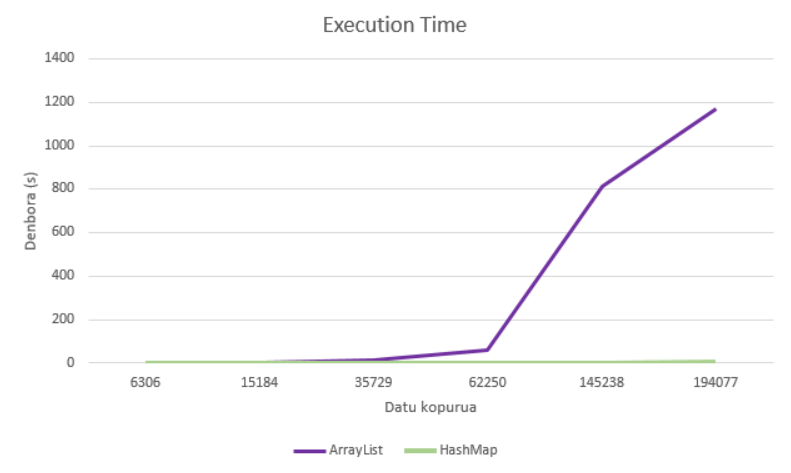
\includegraphics[width=1\textwidth]{ArrayList_Hash_KonparaketaGrafikoa.png}
	\captionof{figure}{ArrayList eta Hash taularen konparaketa grafikoa}

\section{Quick Sort algoritmoaren exekuzio denbora milisegunduetan (ms)}
\begin{table}[h!]
	\begin{scriptsize}
		\begin{center}
			\begin{tabular}{|c|c|c|c|c|c|c|}
				\hline
				\multicolumn{7}{|c|}{Quick Sort algoritmoaren probak milisegunduetan (ms)}\tabularnewline
				\hline 
				\textbf{Fitxategi kop.} & \textbf{1.proba} & \textbf{2.Proba} & \textbf{3.Proba} & \textbf{4.Proba} & \textbf{5.Proba} & $\bar{X}_{QuickSort}$ \\
				\hline
				1 & 0.44 & 0.34 & 0.38 & 0.35 & 0.39 & 0.38  \\
				\hline
				6 & 1.19 & 0.7 & 0.68 & 0.65 & 0.71 & 0.786 \\
				\hline
				11 & 0.88 & 1.04 & 0.83 & 0.85 & 0.81 & 0.882 \\
				\hline
				21 & 1.21 & 1.32 & 1.2 & 1.26 & 1.3 & 1.258 \\
				\hline
				41 & 2.32 & 2.15 & 2.16 & 2.23 & 2.2 & 2.212 \\
				\hline
				54 & 2.77 & 3.00 & 3.12 & 2.96 & 3.04 & 2.978 \\
				\hline
	\end{tabular}\end{center}\end{scriptsize}
	\caption{\label{tab3} Quick Sort algoritmoaren proba bakoitzaren emaitza eta haien batazbestekoa
	}
	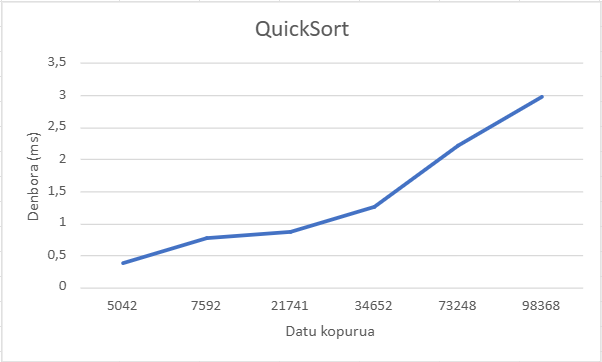
\includegraphics[width=1\textwidth]{QuickSortGrafikoa.png}
	\captionof{figure}{Quick Sort algoritmoaren exekuzio-denbora grafikoki}
	
\end{table}

\end{document}          
